\section{Implementacja}

\begin{frame}<-5>[label=implementation]
    \frametitle{Implementacja}
    \begin{enumerate}
        \item<1-> Analiza teoretyczna
            \begin{itemize}
                \item<2-> jaki efekt chcemy osiągnąć?
                \item<3-> jakie mamy ograniczenia?
                \item<4-> jakich narzędzi możemy użyć?
            \end{itemize}
        \item<5-> Rozbicie zadania na podproblemy
        \item<6-> Ustalenie konwencji dotyczących tworzenia kodu
        \item<7-> Ciągłe testowanie oprogramowania
            \begin{itemize}
                \item<8-> testy jednostkowe
                \item<9-> scenariusze testowe
            \end{itemize}
    \end{enumerate} 
\end{frame}

\begin{frame}{Implementacja}
    \begin{figure}
        \centering
        
\includegraphics[scale=0.5]{img/modularity.png}
    \end{figure}
\end{frame}

\againframe<5-6>{implementation}

\begin{frame}{Implementacja}
    \begin{figure}
        \centering
        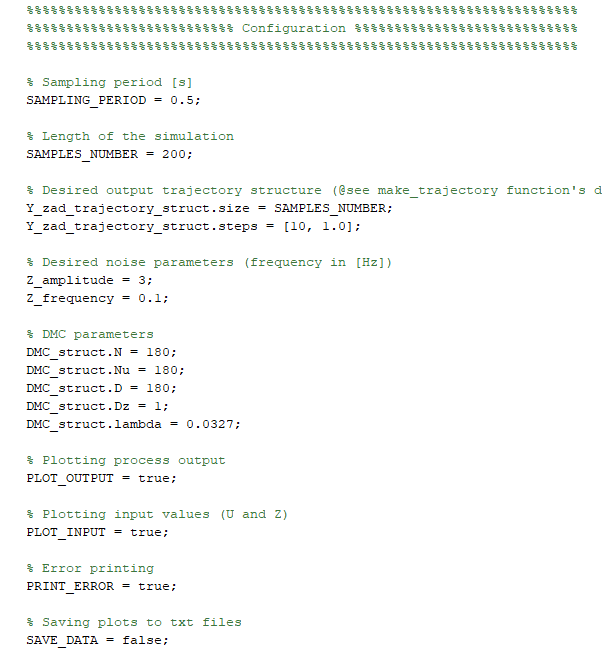
\includegraphics[scale=0.4]{img/Sekcja konfiguracyjna.PNG}
        \caption{Przykładowa sekcja konfiguracyjna}
    \end{figure}
\end{frame}

\againframe<6->{implementation}